\chapter{Descripción das Características}
\label{chap:DescripciónDasCaracteristicas}

\section{\textit{TIBCO Cloud Integration Marketplace}}

\textit{TIBCO Cloud Integration} ten un espazo denominado «\textit{Marketplace}» onde ofrece acceso a conectores, complementos, extensións, aplicacións e aceleradores. Todas estas contribucións están desenvolvidas e proporcionadas por TIBCO, os socios de TIBCO, os provedores de software independentes e os usuarios de \textit{TIBCO Cloud Integration} para axudar cos proxectos de integración de outros usuarios.

A \textit{Marketplace App Listing} é unha plataforma para compartir aplicacións de \textit{TIBCO Cloud Integration - Connect}, \textit{TIBCO Flogo}, o \textit{TIBCO BusinessWorks} con outros usuarios. Cando se crea unha «\textit{Marketplace App Listing}» estase creando unha entrada no mercado de aplicacións de \textit{TIBCO Cloud Integration} onde se inclúe información da aplicación.

\begin{figure}[!ht]
	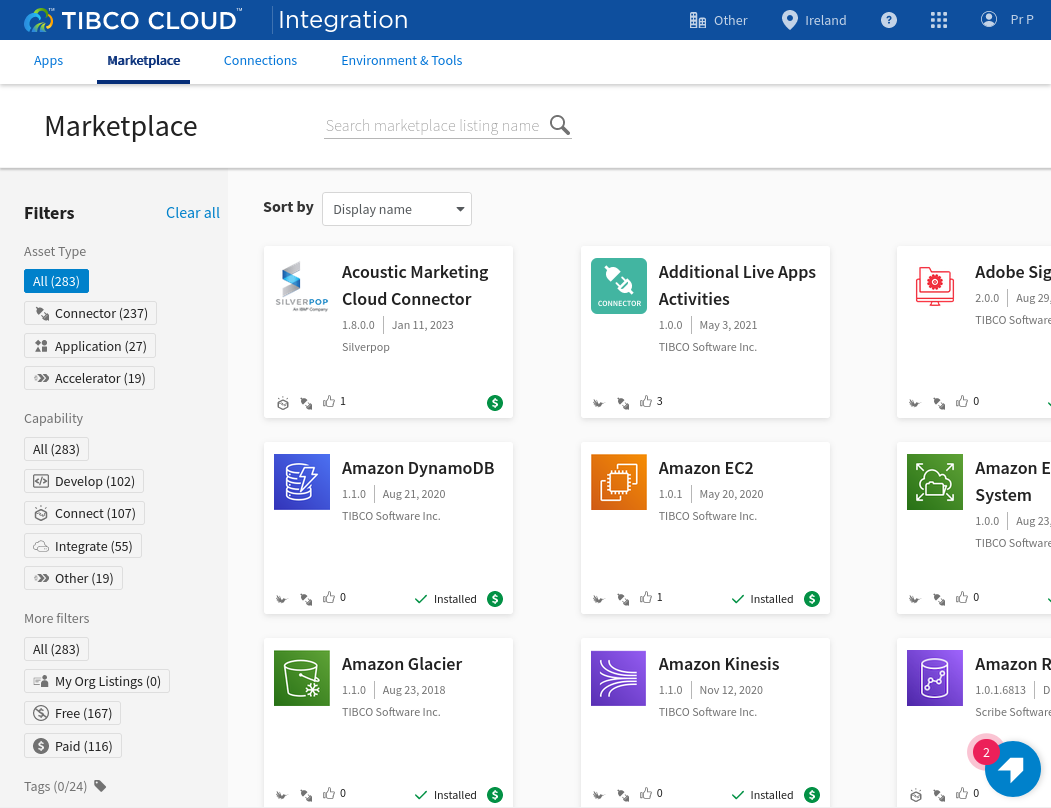
\includegraphics[width=\textwidth]{img/marketplace.png}
	\caption{Páxina do \textit{Marketplace}}
	\label{fig:marketplace}
\end{figure}

Existen dous tipos:

\begin{description}
    \item[Privados] Só visibles para usuarios da túa organización.
    \item[Públicos] Visibles para todos os usuarios de TIBCO Cloud Integration.
\end{description}

\subsection{Crear un App Listing}

\begin{enumerate}
	\item Navega ata a páxina denominada Lista de Aplicacións (\textit{Apps List}) e abre a aplicación  \textit{TIBCO Flogo} ou \textit{TIBCO Cloud Integration - Connect} que queres engadir ao \textit{Marketplace}.
	
	\item Na páxina de detalles da aplicación (\textit{App Details}) seleccione a opción «\textit{Add Market Listing}» situado xunto ao nome da aplicación na parte superior da páxina.
	
	\item Completa os campos e selecciona «\textit{Publish publicly}» para mandala ao \textit{Marketplace}. (Por defecto todos os novos \textit{listings} engádense como privados).
\end{enumerate}

Cando se crea unha aplicación o nome da organización é usado automaticamente no \textit{listing}: se despois o nome da organización muda este campo non estará actualizado.

As aplicacións do \textit{Marketplace} pódense instalar na organización para usalos en integracións propias.

Pódese:

\begin{itemize}
    \item Instalar a App directamente dende o \textit{Marketplace}.
    \item Usar a utilizade de «\textit{Create App}» accesible dende a \textit{Apps List}.
\end{itemize}

Consideracións:

\begin{itemize}
    \item Cando se obtén unha app dende o \textit{Marketplace}, mostrase na listaxe de aplicacións co mesmo nome que a aplicación usada para crear o \textit{listing}, non o nome propio do \textit{listing}.
    
    \item Obter a mesma aplicación varias veces engadirá un número ao nome da mesma cando  se amose nas \textit{Apps Listing}.
    
    \item Despois da instalación da app na organización, deberíanse abrir e actualizar manualmente as conexións de esquemas, as URL das API, etc.
\end{itemize}

\subsection{Obtención dunha App}

Navegar ata o \textit{Marketplace} e  selecciona o \textit{listing} que se desexa instalar. No panel dereito, seleccionar \texttt{GET} ou \texttt{REQUEST}, dependendo de como o provedor configurara o \textit{listing}.

\begin{description}
    \item[GET] instala a app inmediatamente.
    \item[REQUEST] mandase unha petición de acceso ao provedor. Se o provedor acepta a petición o botón cambiase a GET e xa se pode instalar a aplicación.
\end{description}

Despois de seleccionar GET para instalar a app, aparece un pop-up dicindo que unha copia da app será instalada na organización, ademais de alertar sobre a información que será recollida e compartida co provedor da app.

Para rematar, aceptar os termos e Crear a app (que agora mostrarase na \textit{Apps Lists}), e na \textit{Apps List} seleccionar unha nova app e completar a configuración.

\section{Integración dirixida por API}

    A integración dirixida por API é un enfoque da integración que se centra no uso das APIs para conectar aplicacións e datos. Coa integración dirixida por API, as empresas poden aproveitar as vantaxes das APIs para conectar aplicacións de forma rápida e sinxela, independentemente de onde se sitúen esas aplicacións.
   
\subsection{Funcionamento}

\begin{enumerate}
    \item O desenvolvedor crea unha app de integración que utiliza APIs para conectarse ás aplicacións que desexa integrar.
    \item A aplicación de integración utiliza as APIs para intercambiar datos entre as aplicacións.
    \item A aplicación de integración pode utilizar outros compoñentes, como fluxos de traballo, para automatizar tarefas e engadir funcionalidades adicionais.
\end{enumerate}

\subsection{Vantaxes}

\begin{description}
    \item[Velocidade:] Como xa se mencionou anteriormente, a integración dirixida pode axudar as empresas a conectar aplicacións de forma rápida e sinxela.
    \item[Flexibilidade:] Pode utilizarse para conectar aplicacións de calquera tipo, independentemente de onde se encontren.
    \item[Reusabilidade:] As APIs poden reutilizarse en diferentes integracións, o que pode axudar ás empresas a aforrar tempo e custos. 
\end{description}

\subsection{Para que se pode utilizar}

\begin{description}
    \item[Integración de aplicacions na nube:] A integración dirixida por APIs pode utilizarse para conectar aplicacións na nube. Exemplo: AWS, Salesforce...
    
    \item[Integración de datos:] A integración dirixida por APIs pode utilizarse para integrar datos pertencentes a diferentes fontes. Exemplos: Bases de datos, ficheiros...
\end{description}

\section{\textit{TIBCO Cloud Integration - API Modeler}}

\textit{API Modeler} é unha ferramenta web sinxela de usar que permite crear e modelar APIs REST de forma visual.

\subsection{Características principais:}

\begin{description}
    \item[Importar e editar especificacións de APIs:] Importa sen problemas especificacións de API REST existentes en formato YAML o JSON para o seu posterior refinamento e edición.
    
    \item[Modelo Visual de API:] Utiliza a intuitiva interface visual para o modelaxe da API REST, incluídas as definicións de recursos, operacións e tipos de datos.
    
    \item[Mocking e Implementacion de APIs:] Aproveita a función de \textit{mocking} da API para simular o comportamento de API antes de despregala, asegurando a súa funcionalidade.
\end{description}

\section{\textit{TIBCO Cloud Integration - API Mock App}}

Unha aplicación \textit{API Mock} é unha maqueta dunha aplicación que se crea a partir dunha especificación de API existente. Utilizase para simular o comportamento dunha API. 

\subsection{Obxectivo}

\begin{description}
    \item[Probas de Integración:] Pódese utilizar para probar integracións que utilizan APIs. Esto pode axudar a garantir que as integracións funcionen correctamente.
    \item[Desenvolvemento de Integracións:] Pódese utilizar para o desenvolvemento de integracións que utilizan APIs para axudar a crear integracións máis rapidamente e reducir o risco de erros.
\end{description}

\subsection{Compoñentes}

\begin{description}
    \item[Endpoints:] Enderezo URL que se utiliza para acceder á API \textit{Mock App}.
    \item[Definición de API:] A definición de API especifica os métodos da API, os parámetros que aceptan e os datos que devolven.
    \item[Implementación da API:] Código que implementa os métodos da API.
\end{description}

\section{Integración dirixida por eventos}

A Integración dirixida por eventos é un enfoque que se centra no uso de eventos para conectar aplicacións e datos. As empresas poden aproveitar as vantaxes dos eventos para conectar de forma rápida e sinxela, independentemente de onde se encontren estas aplicacións.

\textit{TIBCO Cloud Integration} prové unha gran variedade de funcionalidades que facilitan a integración dirixida por eventos:

\begin{itemize}
    \item Moitos tipos de eventos.
    \item Ferramenta de desenvolvemento de eventos: Estas ferramentas axudan aos desenvolvedores a crear eventos seguros, escalables e doados de usar.
    \item Xestión de eventos: Facilitan o control, mantemento e a administración de eventos garantindo que sexan seguros e eficaces.
\end{itemize}

\subsection{Funcionamento}

\begin{enumerate}
    \item O desenvolvedor crea o evento que se utiliza para conectar as aplicacións que desexa integrar. Un evento é unha mensaxe que conten información sobre un cambio que se produciu nunha aplicación ou sistema. O evento pode conter información sobre o tipo de cambio, a data e hora ou os datos afectados.
    
    Para a creación deste evento pódese utilizar a ferramenta de desenvolvemento de eventos de \textit{TIBCO Cloud Integration} que ten interface gráfica.
    
    \item O evento publicase nun bus de eventos, é dicir, nun servizo que permite as aplicacións intercambiar eventos.
    
    Concretamente o bus de eventos de \textit{TIBCO Cloud Integration} denominase \textit{Event Broker}.
    
    \item As aplicacións que están subscritas ao bus de eventos reciben o evento. Isto realizase na ferramenta de de desenvolvemento de fluxos de integración.
    
    \item As aplicacións procesan o evento realizando acción en función dos seus contidos. Isto tamén realizase coa ferramenta de desenvolvemento de fluxos de integración.
\end{enumerate}

\section{Fluxos de Integración nativos na nube}

\textit{TIBCO Cloud Integration} ofrece moitos tipos de funcionalidades para crear e xestionar fluxos de integración nativos na nube.

\begin{figure}[!ht]
	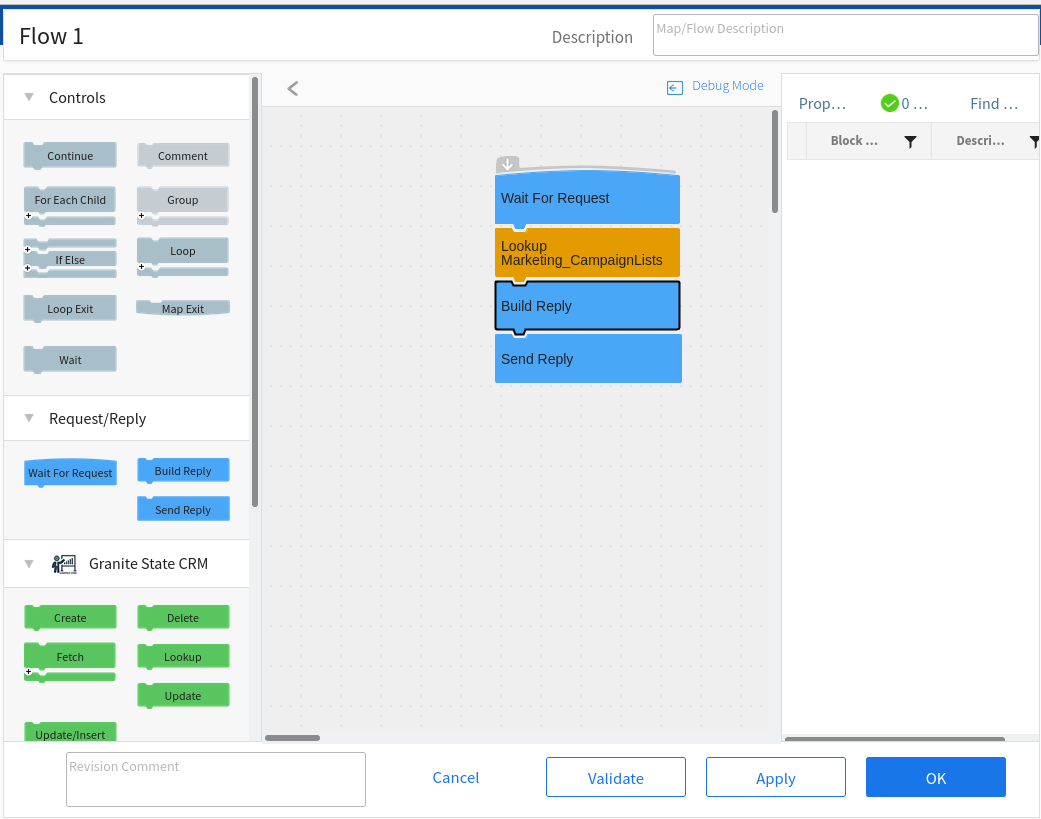
\includegraphics[width=\textwidth]{img/fluxo.png}
	\caption{Interface de fluxo}
	\label{fig:fluxo}
\end{figure}

\subsection{Creación de fluxos de Integración}

A creación de fluxos de integración é un proceso sinxelo que se pode realizar mediante unha interface de usuario intuitiva. Os fluxos de integración pódense crear a partir dun modelo ou desde cero.

Os modelos proporcionan un punto de partida para crear fluxos de integracións comúns. Por exemplo, existen modelos dispoñibles para replicar datos e integrar aplicacións ou procesar eventos.

\subsection{Transformacións de datos}

\textit{TIBCO Cloud Integration} ten unha variedade de funcións de transformacións de datos, como poden ser limpeza, transformación e validación. Permiten garantir a calidade de datos que se moven a través dos fluxos de integración.

\subsection{Encamiñamento de datos}

\textit{TIBCO Cloud Integration} permite encamiñar os datos a través dunha variedade de destinos, como aplicacións, bases de datos, servizos na nube ou sistemas de almacenamento.

O encamiñamento pódese configurar utilizando regras ou funcións. As regras utilízanse para encamiñar os datos en función de criterios específicos e as funcións utilízanse para encamiñar os datos en función da lóxica definida polo usuario.

\subsection{Control e Xestión}

\textit{TIBCO Cloud Integration} ten unha gran variedade de capacidades de control e xestión, o que lles permite aos usuarios supervisar o rendemento dos fluxos de integración e solucionar problemas.

\section{\textit{TIBCO Cloud Integration - Connect}}

\textit{TIBCO Cloud Integration - Connect} é  unha solución de integración de datos que permite a conectividade sen problemas entre aplicacións baseadas na nube e locais.

Os integradores teñen a capacidade de crear e administrar integracións de datos robustas cunha interface de usuario doada de entender e un conxunto completo de conectores.

\subsection{Compoñentes Principais}

\begin{description}
    \item[Motor de Integración:] Corazón de \textit{TIBCO Cloud Integration - Connect}, responsable de dirixir o movemento de datos entre aplicacións de fontes de datos.
    
    Encargase das transformacións complexas, manexo de erros e encamiñamento de datos.
    
    \item[Conectores:] Prové conectividade lista para usar nunha gran gama de aplicacións, bases de datos e plataformas na nube. Cada conector encapsula os protocolos de comunicación e formatos de datos específicos do sistema conectado.
    
    \item[Axente:] Compoñente do software local instalado que facilita a comunicación segura entre \textit{TIBCO Cloud Integration - Connect} na nube e as fontes de datos locais. Garante a seguridade dos datos e o cumprimento das políticas das devasas.
\end{description}

\subsection{Vantaxes}

\begin{description}
    \item[Conectividade Amplia:] admite unha ampla gama de aplicacións, bases de datos e plataformas na nube, o que permite unha integración sen problemas en ambientes de TI diversos.
    
    \item[Mellora da calidade dos datos:] Facilita a limpeza de datos, transformación e validación para garantir a precisión e consistencia dos datos nos sistemas.
    
    \item[Reducción dos costos de integración:] Elimina a necesidade da manipulación manual dos datos e reduce o tempo e os recursos necesarios para o mantemento da integración.
    
    \item[Escalabilidade:] Admite volumes crecentes de datos complexos, asegurando que a integración de datos pode escalar cuns requisitos comerciais en evolución.
\end{description}
